\documentclass[]{article}

\usepackage{amsmath}  % AMS math package
\usepackage{amssymb}  % AMS symbol package
\usepackage{bm}       % bold math
\usepackage{graphicx} % Include figure files
\usepackage{dcolumn}  % Align table columns on decimal point
\usepackage{multirow} % Multirow/column tables
\usepackage{hyperref} % Hyperlinks

\begin{document}

\title{Three-Dimensional Molecular Dynamics Simulation:\\with Verlet algorithm}% Force line breaks with \\
\author{Tridip Das}
\date{March 31, 2015}% It is always \today, today, but you can specify other dates manually 
\maketitle

\begin{abstract}
The study of classical Molecular Dynamics investigates the interaction of atoms in a face centered cubic (FCC) lattice at different temperature.
For this study Newton's law of particle interaction has been applied with Verlet algorithm for velocity calculation. The potential interactions are described
with Lennard-Jones pair potential. For initialization of velocity Box-Muller method is used. The particles are interacted in periodic boundary conditon.
864 atoms are taken for all the studies described, which is sufficient to adequately describe the system. The temperature effect on lattice is studied with radial distribution function, which shows melting phenomena. For ease of calculation scaled parameters are used in this study.
\end{abstract}

\section{Introduction} %Title for the section
\label{sec:level1} %Label for the section, to be used for referencing in other parts of the document
The study of Molecular Dynamics (MD) investigates the interaction and motion of atoms/molecules in a many body simulation. The concept of MD applicable in wide area of sciences. Though there are two types of MD simulations ab initio and classic, this study investigates the classical version. The classical MD concept stands on famous Newton's equation $F = ma$. We just solve this equation with applied mathematical concepts.

\begin{equation}
\label{eq:one} %Label for the equation, to be used for referencing in other parts of the document
  \overrightarrow{F} = m \overrightarrow{a} = m \frac{{d}^2 \overrightarrow{r}} {d {t}^2}
\end{equation}


\section{Simulation Methodology}
Though the classical MD sounds pretty simple as it requires to solve $ F = ma $ but the algorithmic methods developed to attain this simple problem are interesting.
\\
\subsection{Initial velocity with Box-Muller}
In the Box-Muller method random rumbers are used between [0,1]. Two random numbers $x_1$ and $x_2$ are generated. They are used in below equations to calculate velocity.
\begin{equation} 
  v_1 = \sqrt{-2 ln x_1} cos(2\pi x_2)
\end{equation}
\begin{equation} 
  v_2 = \sqrt{-2 ln x_2} sin(2\pi x_1)
\end{equation}
\\
Velocities can be choosen using Maxwell-Boltzmann distribution
\begin{equation} 
  P(\overrightarrow{v}) = {(\frac{m}{2\pi k_B T})}^{\frac{3}{2}} exp[-\frac{m({v_x}^2+{v_y}^2+{v_z}^2)}{2 k_B T}]
\end{equation}
\\
\subsection{Lennard Jones potential}
The interatomic potential between two particle is calculated using Lennard Jones pair potential. The minimum distance between atoms are set by $r_{min} = 2^{\frac{1}{6}}\sigma$ and depth of the minimum as $-\epsilon$. All parameters are scaled as $ m = 1, \sigma = 1, \epsilon = 1 $. Again one unit of time scale for this problem is $\tau = (\frac{m {\sigma}^2}{\epsilon}) = 2.17ps$. So, the simulation is executed for $4.34ps$ to observe steady state effect with a time step of $2.17fs$.
\begin{equation} 
  V(r) = 4\epsilon[{(\frac{\sigma}{r})}^{12} - {(\frac{\sigma}{r})}^{6}]
\end{equation}
\\
The Force is calculated as:
\begin{equation} 
  \overrightarrow{F}(r) = -\frac{\partial V}{\partial r} \hat{r}
\end{equation}
\\
\subsection{The Verlet algorithm}
The Verlet algorithm solves the differential form of velocity and acceleration with numerical approach. Finite difference methods can be used for the purpose. As in central difference method the correction term, $ O { (\delta t)}^{2}$ is of higher order than forward and backward difference method, $ O  (\delta t)$, the cetral difference formula is employed to develop Verlet equations to calculate velocity and displacement:
\begin{equation} 
  \overrightarrow{v_i} (t+\delta t) = \overrightarrow{v_i}(t) +  \frac{1}{2}\delta {t}(\overrightarrow{a_i}(t + \delta t) + \overrightarrow{a_i}(t))
\end{equation}
\begin{equation} 
  \overrightarrow{x_i} (t+\delta t) = \overrightarrow{x_i}(t) + \delta t \overrightarrow{v_i}(t) + \frac{1}{2}\delta {t}^{2}\overrightarrow{F_i}(t)/m_i
\end{equation}
\\
The temperature correction of velocity is performed according to below formula to check the run away of the particles.
\begin{equation} 
  \overrightarrow{v}_{new}  = \overrightarrow{v_i} \sqrt{\frac{T_{goal}}{T_{simulated}}}
\end{equation}
\section{Results}
The classical Molecular Dynamics simulation is implemented in Python and Fortran. The FCC lattice generation part is done in Python then Fortran is used for all the calculations. Again Python is used to generate all the plots. Fortran is used for velocity initialization to final energy and lattice position calculations. Code is available in github at \url{https://github.com/tridip66/molecular_dynamics/tree/master/src}. The simulation tries to keep the temperature constant, so steady kinetic energy is observed. The total energy of the system fluctuates around a steady state but it may subside with much bigger system. It can be observed in the Figure 1 which is ran for $ 4.34ps$ at $T = 1$. For visualization of crystal lattice VESTA has been used.
\\
\begin{figure}[ht]
  \centering
  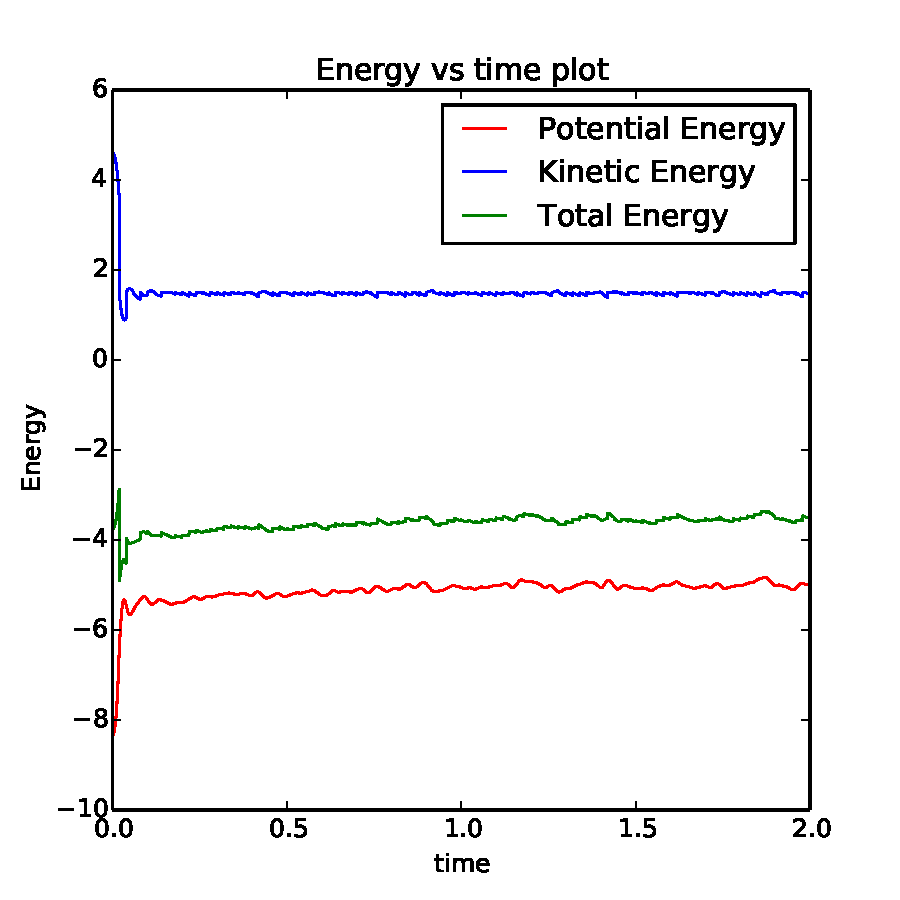
\includegraphics[scale=0.4]{figures/EnergyPlot}% Imports a figure - does not automatically scale
  \caption{\label{fig:epsart} Energy vs time plot at T = 0.1 for 4.34 ps of simulation}
\end{figure}
\\
The temperature fluctuation with simulation time is shown in Figure 2. The goal for temperature was set at T = 1.0. The temperature varies nicely around the goal.
\\
\begin{figure}[ht]
  \centering
  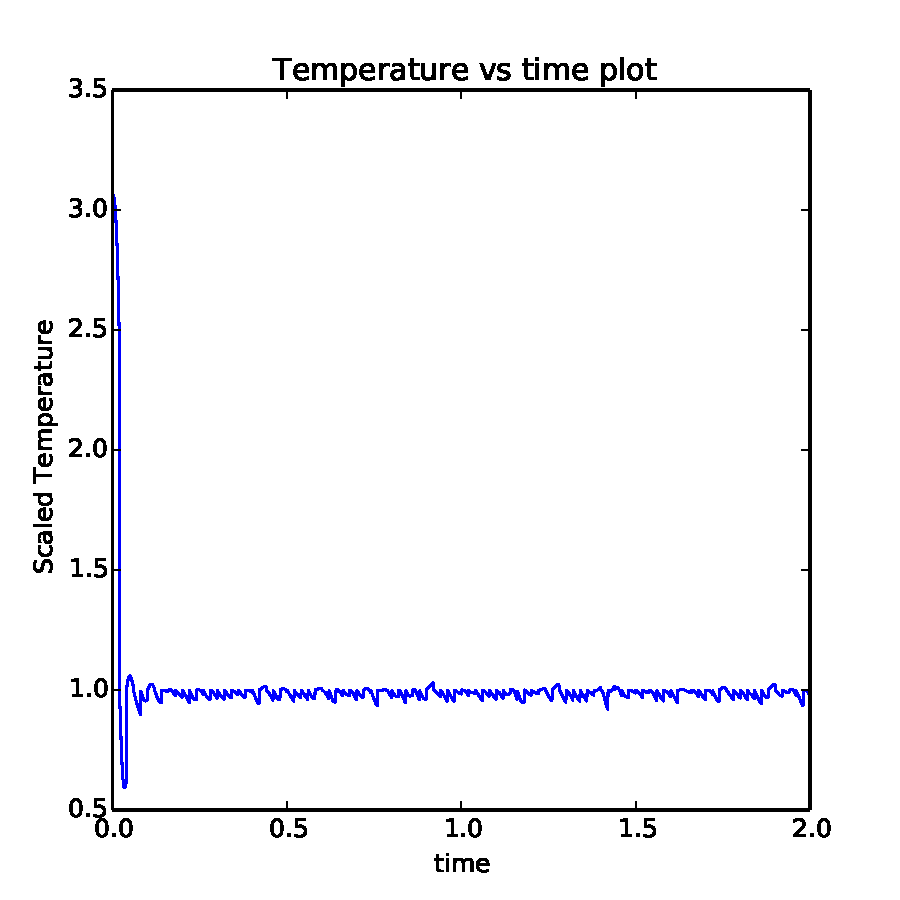
\includegraphics[scale=0.5]{figures/TempPlot}% Imports a figure - does not automatically scale
  \caption{\label{fig:epsart} Temperature fuctuation around T = 1.0 with time calculated at T = 1.0}
\end{figure}
\\
The pressure fluctuation with simulation time is shown in Figure 3.
\\
\begin{figure}[ht]
  \centering
  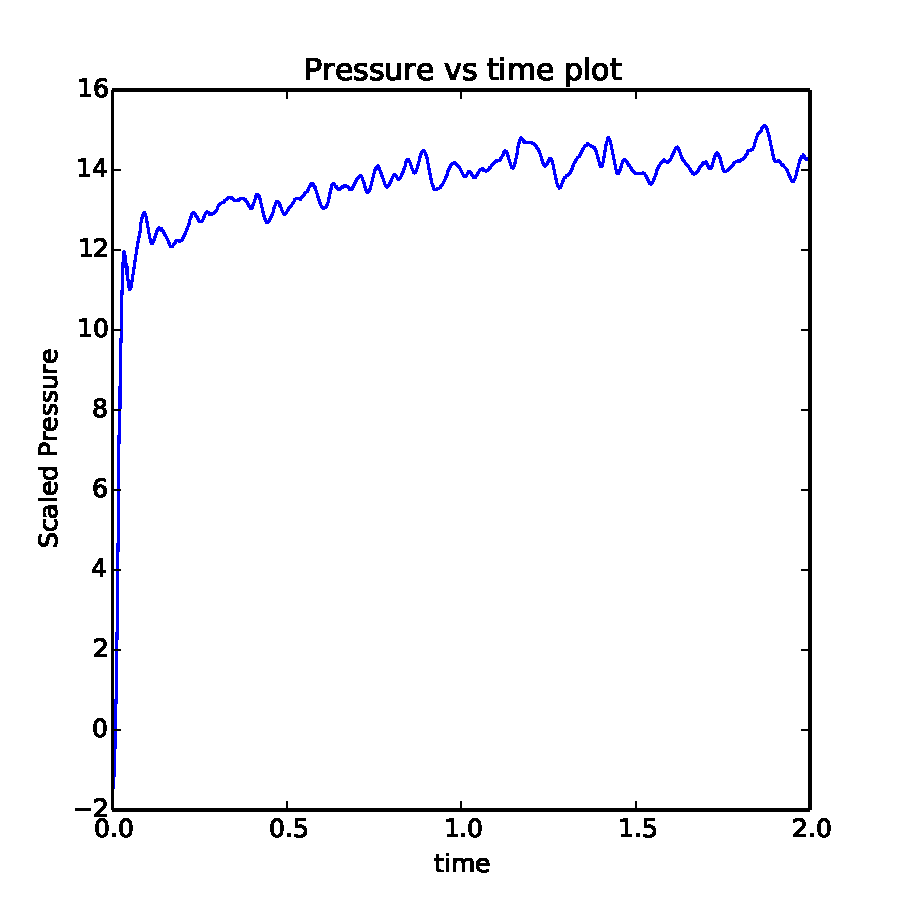
\includegraphics[scale=0.5]{figures/PressurePlot}% Imports a figure - does not automatically scale
  \caption{\label{fig:epsart} Pressure fuctuation with time calculated at T = 1.0}
\end{figure}
\\
During the simulation of the FCC lattice it was possible that due to resultant velocity of all the particles the simulation box may get some momentum. Hence, a correction has been applied for the velocity to keep the momentum of the center of mass negligible. The momentum of the center mass with time is shown in Figure 4 at high temperature T = 1.0, when the velocity fluctuation is higher.
\begin{figure}[ht]
  \centering
  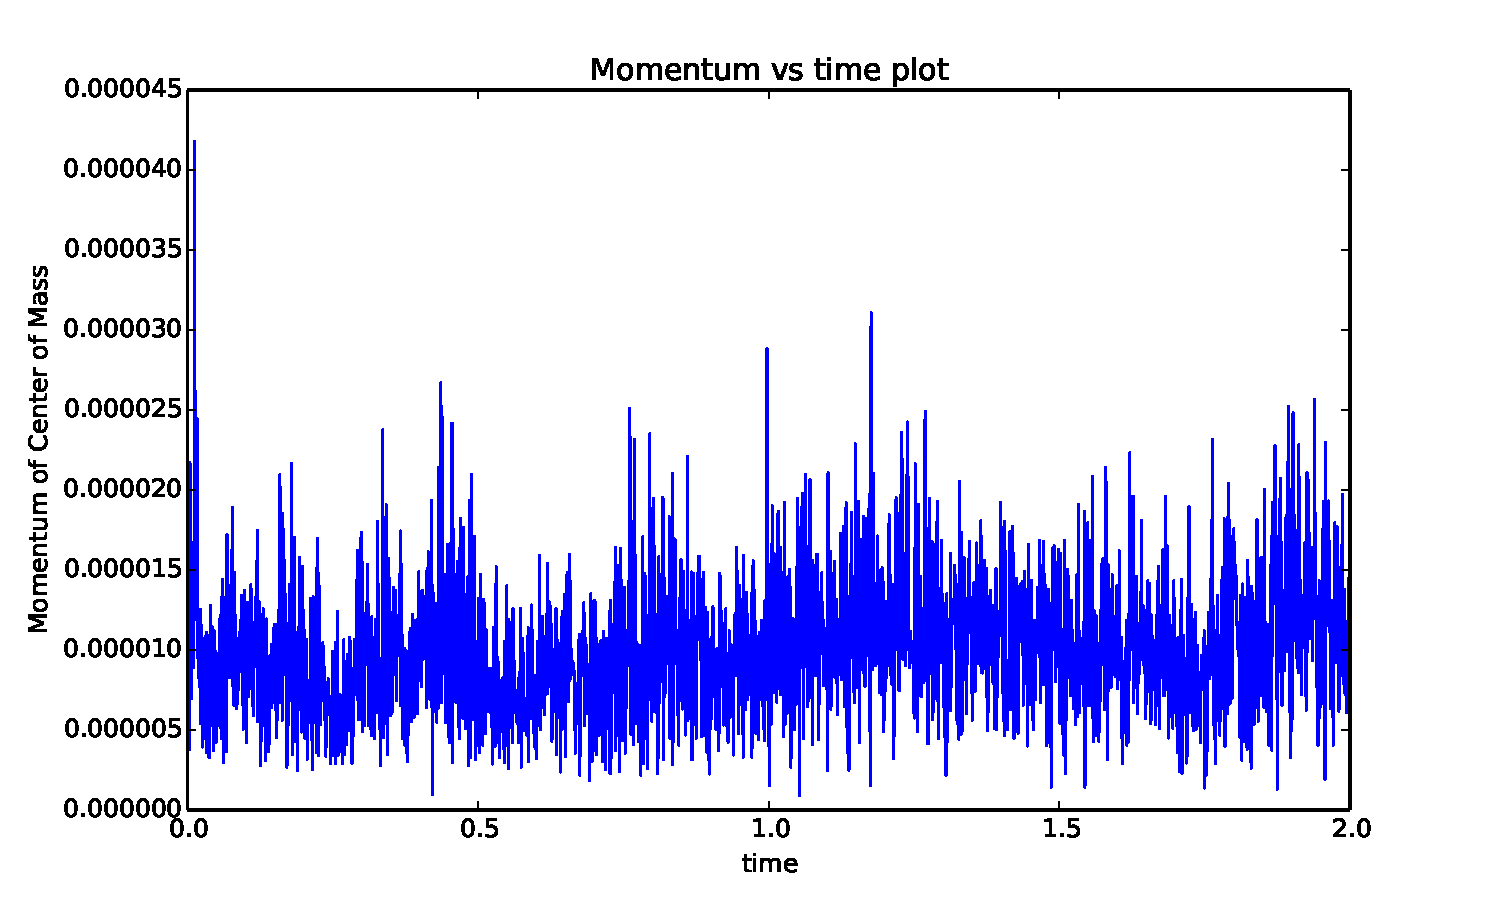
\includegraphics[scale=0.4]{figures/MomPlot}% Imports a figure - does not automatically scale
  \caption{\label{fig:epsart} Momentum of the center of mass with time at T = 1.0}
\end{figure}
\\
As the velocity fluctuation for every particle can be interesting phenomena to observe and it can give an idea of melting when translated to displacement, so the velocity fluctuations of five particles are plotted in Figure 5. Velocity variation with time is not plotted for all the particles as it will make the plot clumsy.
\begin{figure}[ht]
  \centering
  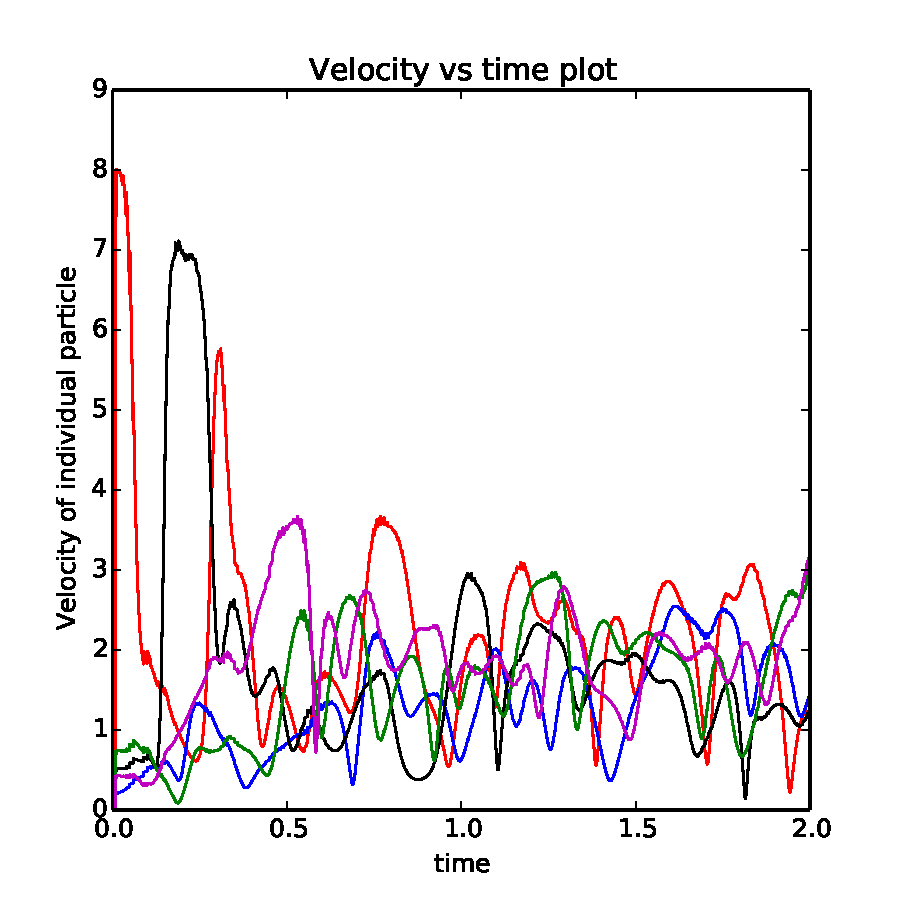
\includegraphics[scale=0.4]{figures/VelPlot}% Imports a figure - does not automatically scale
  \caption{\label{fig:epsart} Velocity fluctuation with time at T=1.0}
\end{figure}
\\
\subsection{Visualization of Melting}
The final position of the atoms in the crystal lattice are recorded after a 4.34 ps of simulation run. As the time is sufficient to reach the steady temperature for the system. In Figure 6 final atom postions are displayed for four different temperatures $ (T = 0.0, 0.1, 0.5, 1.0)$. For simplicity only 32 atoms cell is shown. At temperature $ T = 0.5$ it is clear that lattice vibation increases and at $T = 1.0 $ the periodicity of the system is lost. VESTA is used for the visualization of the structures. For better capturing of melting radial distribution function has been plotted with 864 atoms. The RDF plot at $ T = 0.1 $ in Figure 7 shows the peridocity in the structure. From the RDF plots we can conclude that melting occurs at $ T = 0.8 $
\\
\begin{figure}[ht]
  \centering
  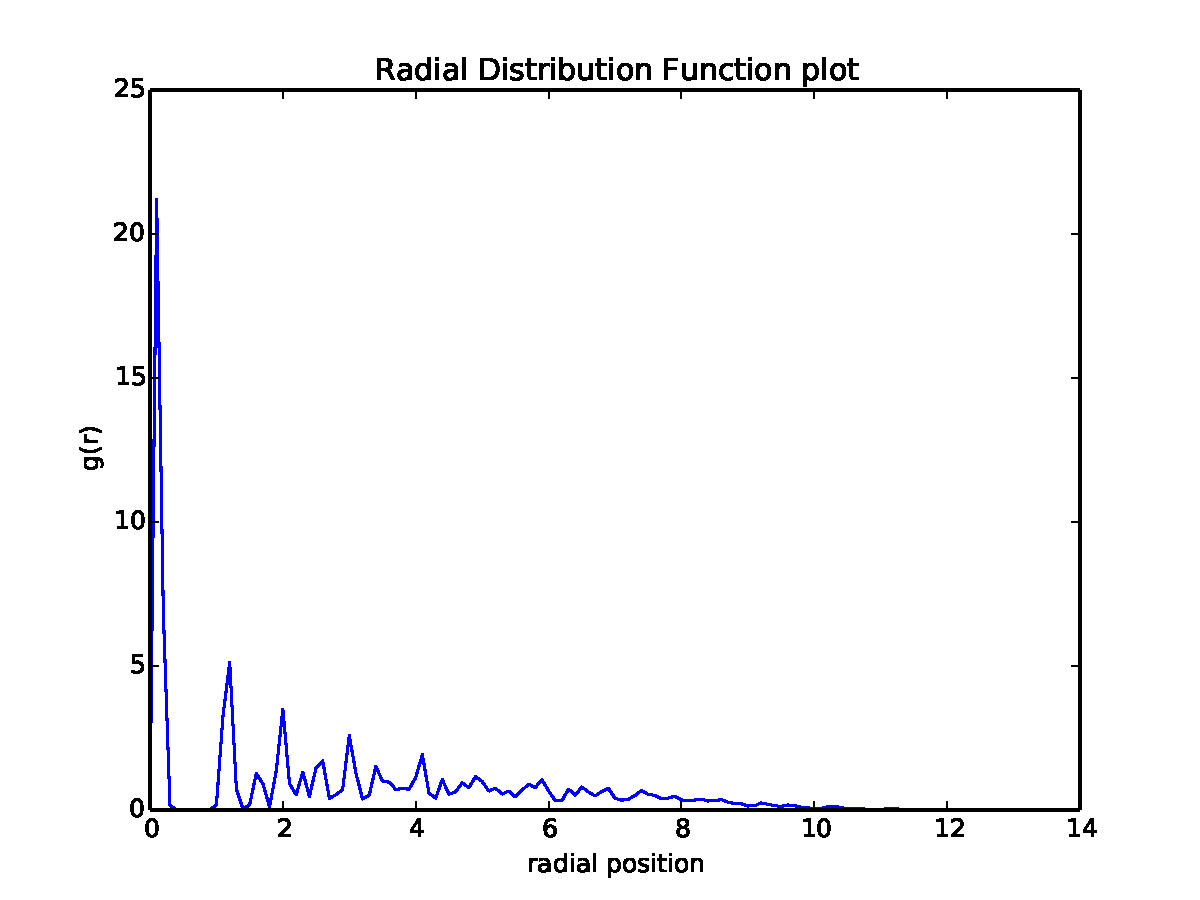
\includegraphics[scale=0.3]{figures/RDFPlot1}% Imports a figure - does not automatically scale
  \caption{\label{fig:epsart} RDF plot at T = 0.1}
\end{figure}
\\
\\
\begin{figure}[ht]
  \centering
  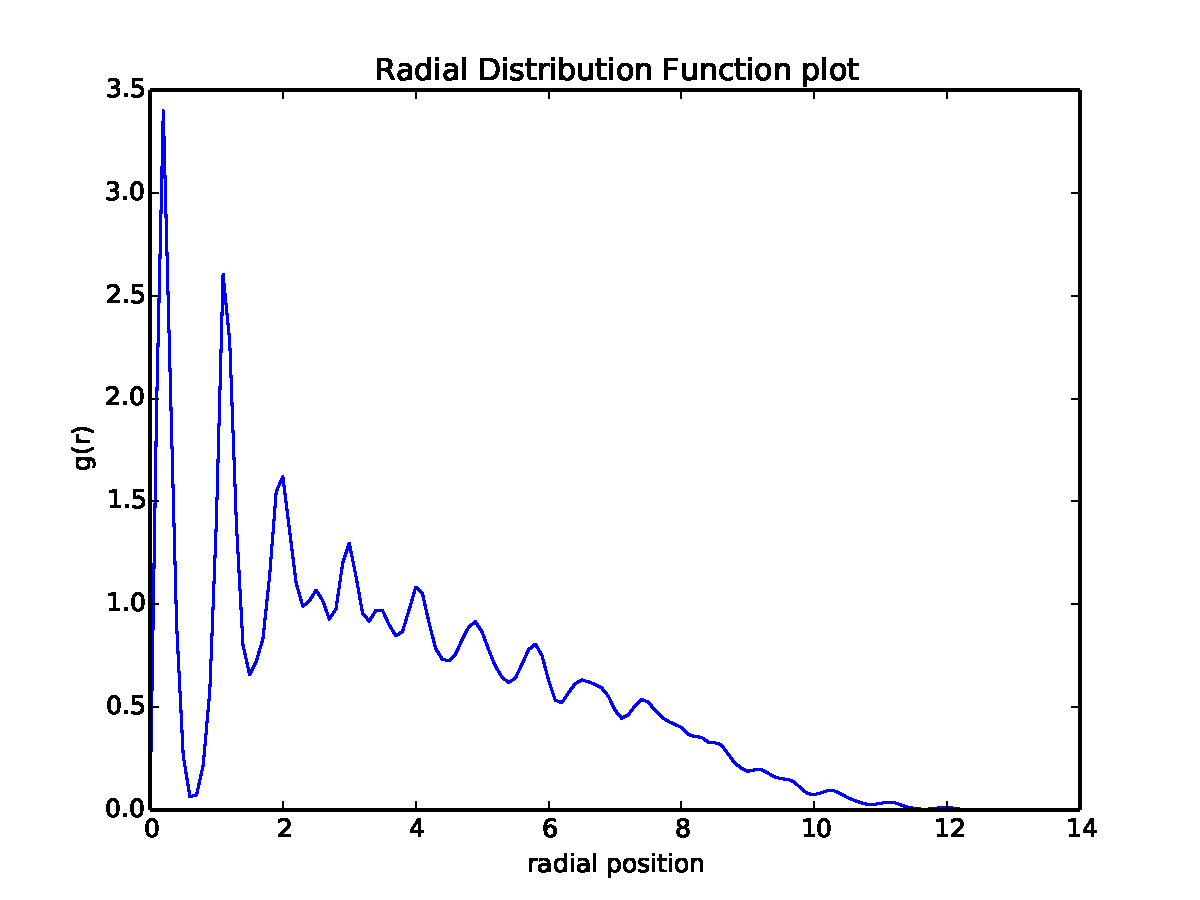
\includegraphics[scale=0.3]{figures/RDFPlot7}% Imports a figure - does not automatically scale
  \caption{\label{fig:epsart} RDF plot at T = 0.7}
\end{figure}
\\
\\
\begin{figure}[ht]
  \centering
  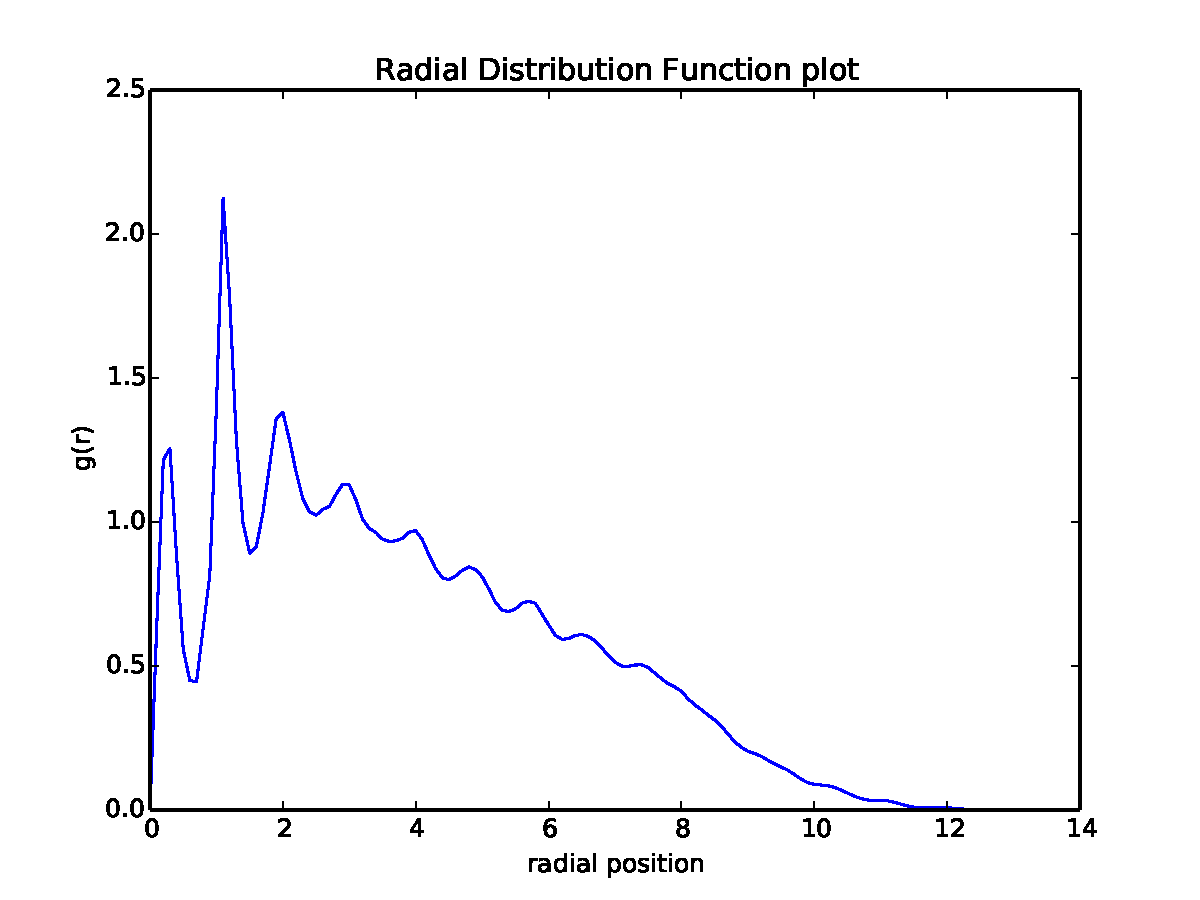
\includegraphics[scale=0.3]{figures/RDFPlot8}% Imports a figure - does not automatically scale
  \caption{\label{fig:epsart} RDF plot at T = 0.8}
\end{figure}
\\
\section*{References}
R. Schneider, A. R. Sharma, and A. Rai, "Introduction to Molecular Dynamics," in Computational Many-Particle Physics, vol. 739, H. Fehske, R. Schneider, and A. Weibe, Eds. Berlin, Heidelberg: Springer Berlin Heidelberg, 2008, pp. 3�40 
\\
\\
Box, G. E. P. and Muller, M. E. "A Note on the Generation of Random Normal Deviates." Ann. Math. Stat. 29, 610-611, 1958.
\\
\\
\url{http://en.wikibooks.org/wiki/LaTeX/Mathematics}
\\
\\
\url{http://en.wikibooks.org/wiki/LaTeX/Importing_Graphics}
\\
\end{document}
